% -*-latex-*-
%
%  For more information, please see: http://software.sci.utah.edu
% 
%  The MIT License
% 
%  Copyright (c) 2004 Scientific Computing and Imaging Institute,
%  University of Utah.
% 
%  License for the specific language governing rights and limitations under
%  Permission is hereby granted, free of charge, to any person obtaining a
%  copy of this software and associated documentation files (the "Software"),
%  to deal in the Software without restriction, including without limitation
%  the rights to use, copy, modify, merge, publish, distribute, sublicense,
%  and/or sell copies of the Software, and to permit persons to whom the
%  Software is furnished to do so, subject to the following conditions:
% 
%  The above copyright notice and this permission notice shall be included
%  in all copies or substantial portions of the Software.
% 
%  THE SOFTWARE IS PROVIDED "AS IS", WITHOUT WARRANTY OF ANY KIND, EXPRESS
%  OR IMPLIED, INCLUDING BUT NOT LIMITED TO THE WARRANTIES OF MERCHANTABILITY,
%  FITNESS FOR A PARTICULAR PURPOSE AND NONINFRINGEMENT. IN NO EVENT SHALL
%  THE AUTHORS OR COPYRIGHT HOLDERS BE LIABLE FOR ANY CLAIM, DAMAGES OR OTHER
%  LIABILITY, WHETHER IN AN ACTION OF CONTRACT, TORT OR OTHERWISE, ARISING
%  FROM, OUT OF OR IN CONNECTION WITH THE SOFTWARE OR THE USE OR OTHER
%  DEALINGS IN THE SOFTWARE.
%


% running.tex
%
% This is the `Running SCIRun' main section.

\chapter{Starting \sr{}}
\label{ch:startingup}


\section{Preparation}
\label{sec:prepare}

Preparations must be made before starting \sr{} and its Power Apps.
Commands below are typed in a terminal emulation application (\eg{}
\command{xterm}).

See \secref{\sr{}'s
Initialization File---\filename{.scirunrc}}{sec:scirunrc} and \secref{Dynamic
Compilation}{sec:dyncomp} for additional information.
  
Mac OSX users must increase the open files limit.
Users of csh-type shells on Mac OSX must type:

\begin{alltt}
  limit descriptors unlimited
\end{alltt}

and users of sh-type shells must type:

\begin{alltt}
  ulimit -n unlimited
\end{alltt}

It is convenient to place the above  in a shell initialization
file (\filename{.cshrc} or \filename{.bashrc}).

%begin{latexonly}
\newcommand{\srwindow}{%
  \centerline{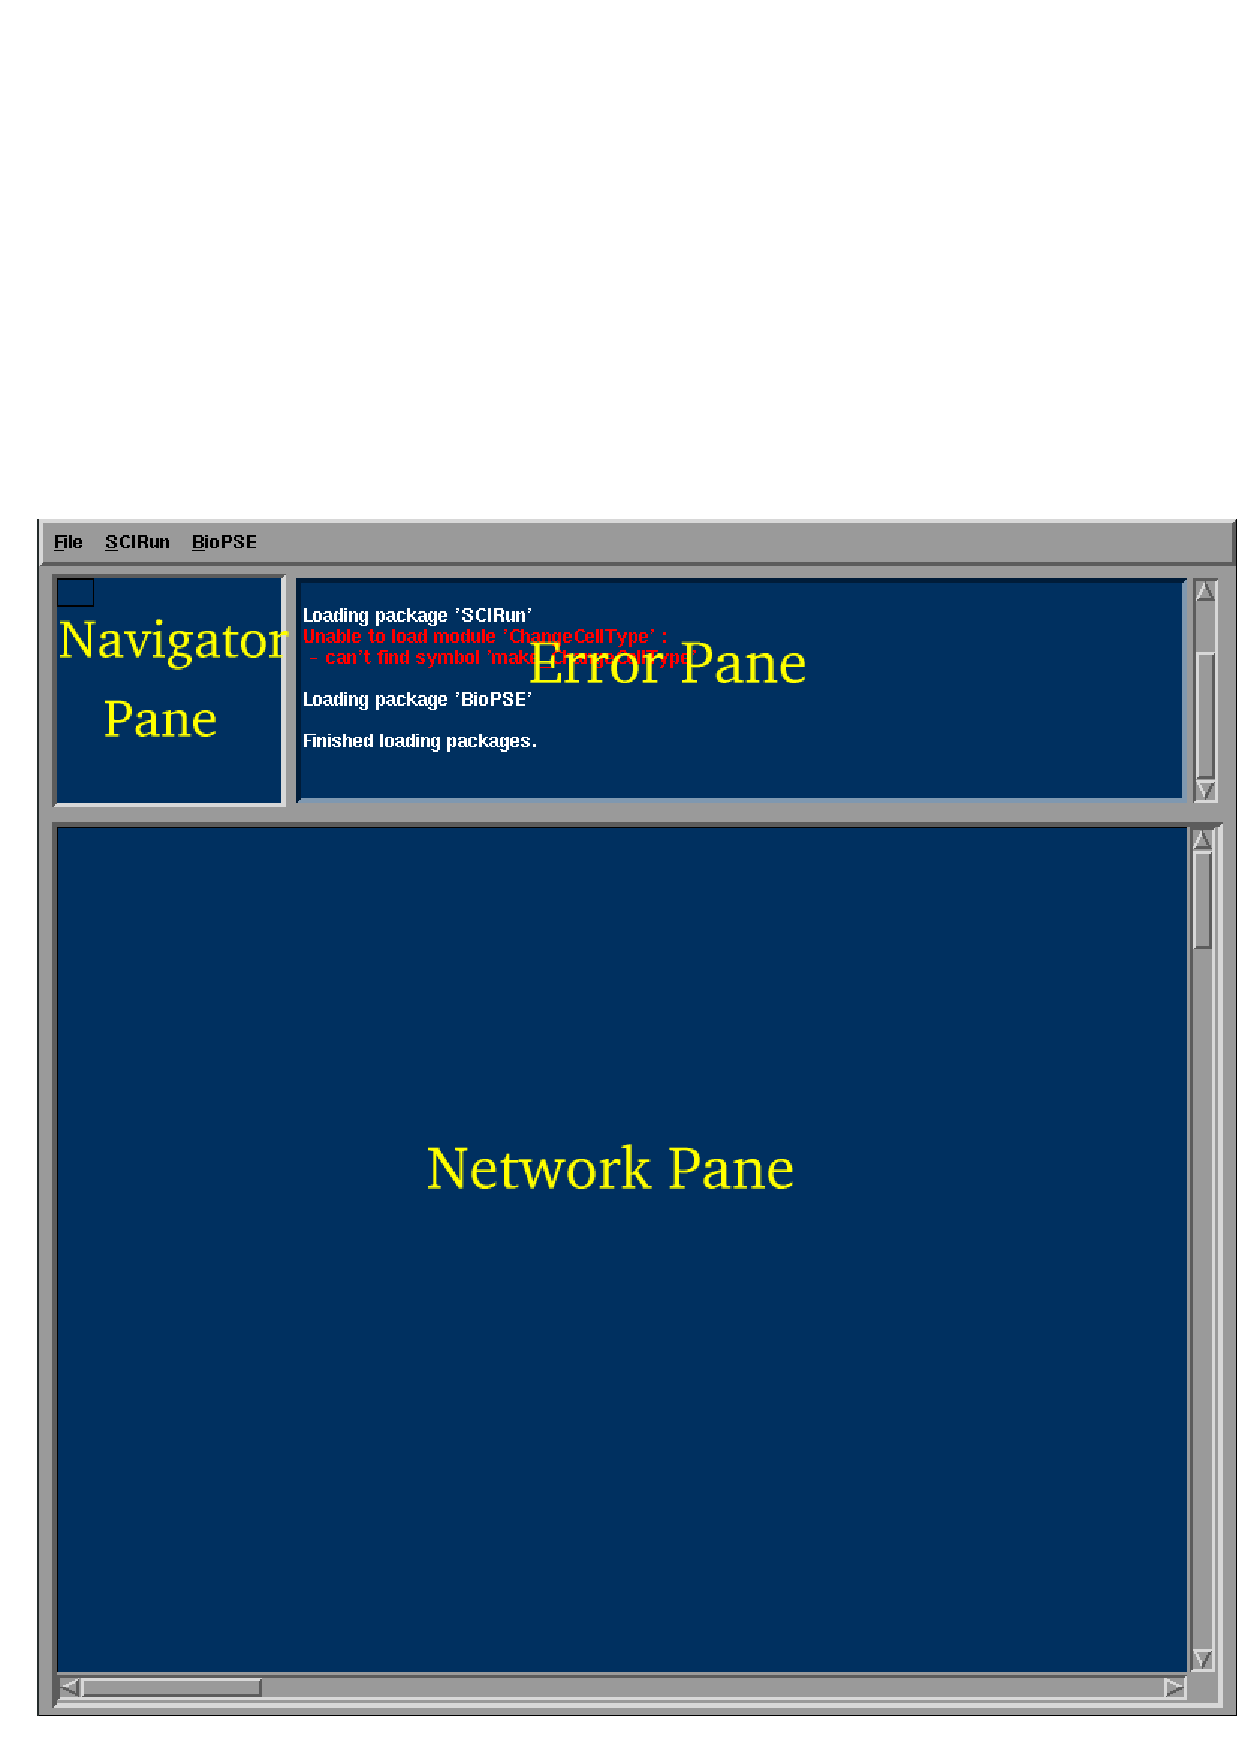
\includegraphics[bb=0 0 400 410,width=6in]{Figures/srwindow-1.eps.gz}}
}
%end{latexonly}
\begin{htmlonly}
  \newcommand{\srwindow}{%
    \htmladdimg[alt="SCIRun Window"]{../Figures/srwindow-1.gif}
  }
\end{htmlonly}

Change your current working directory to \sr{}'s
build directory (for an installation from source code) or to
\filename{/usr/local/SCIRun/bin} (for an installation from an RPM):

\begin{alltt}
  cd SCIRun/sgi32
\end{alltt}

or

\begin{alltt}
  cd /usr/local/SCIRun/bin
\end{alltt}

and type:

\begin{alltt}
  ./scirun [ [-e] \replaceable{network_file} ]
\end{alltt}

\note{Do not start \sr{} in the background, \ie do not type:
  \keyboard{scirun~\&}.}

The \command{scirun} command may take the name of a
\dfn{\sr{} network file} (network files have a \filename{.net} extension)
for \sr{} to load.  The \option{-e} tells \sr{} to execute the network
after it is loaded.  Network files are discussed in a later section.

If the name of a network file is not provided, \sr{} starts with an empty
  window as shown in Figure~\ref{fig:srwindow}.  \secref{Anatomy
  of the Main Window}{sec:windowanatomy} discusses the main features
of Main Window window.

\begin{figure}[htb]
  \begin{makeimage}
  \end{makeimage}
  \srwindow
  \caption{\label{fig:srwindow} \sr{} Main Window}
\end{figure}

\sr{} may encounter errors during start up.  Errors, warnings, and
other messages are displayed in \sr{}'s Message frame (see
Figure~\ref{fig:srwindow}).  Errors should be
\htmladdnormallink{reported}{\bugsurl} to the \sr{} development team
(See \secref{Reporting Bugs}{sec:bugs} for information on reporting
bugs).

\section{Anatomy of the Main Window}
\label{sec:windowanatomy}

The \sr{} main window consists of the Menu Bar, the Global View frame,
the Message frame, and the Net Edit frame (see
Figure~\ref{fig:srwindow}):

\begin{description}
  \descitem{Menu Bar} The menu bar is used to load networks, save
  networks, quit \sr{}, create network modules, and perform other
  tasks.  The menu bar consists of the following menu items:

  \begin{description}
    \menudesc{File} The \menu{File} menu contains the following items:

    \begin{description}
      \menuitemdesc{Load} Loads a network from a file (See
      \hyperref{this section}{Section~}{}{sec:opennet}).
      
      \menuitemdesc{Insert} Adds a network to the NetEdit frame
      without overlap (See \hyperref{this
        section}{Section~}{}{sec:insertnetwork}).
      
      \menuitemdesc{Save} Saves a network to a file (See \hyperref{this
        section}{Section~}{}{sec:savenet}).

      \menuitemdesc{Save As...} Saves a network to a new file (See
      \hyperref{this section}{Section~}{}{sec:savenet}).
      
      \menuitemdesc{Clear Network} Removes all modules and connections from
      the NetEdit frame (See \hyperref{this
        section}{Section~}{}{sec:clearnetwork}).

      \menuitemdesc{Select All} Selects all modules.

      \menuitemdesc{Execute All} Executes all modules.
      
      \menuitemdesc{New} Contains items of interest to
      developers only (e.g. creating new modules).
      
      \menuitemdesc{Add Info} Adds network specific
      notes to the current network.  Notes should be used to document
      the purpose of the network (See \hyperref{this
        section}{Section~}{}{sec:docnetwork}).
    
      \menuitemdesc{Quit} Quits \sr{}.  Pressing key combination
      \keyboard{Control + Q} also quits.
    \end{description}
  \end{description}
  
  \begin{description}
    \menudesc{SCIRun} The \menu{SCIRun} menu is used to create modules
    (from the \sr{} package) for use in the Net Edit frame.

    This menu is composed of sub-menus. Each sub-menu corresponds to
     a \dfn{category}
    \index{category} within the \sr{} package.  A category is a group of
    related modules.  Each menu item in a category sub-menu creates a
    specific module and places it in the NetEdit frame.  
    
    The NetEdit frame pop-up menu  also
    provides access to the \menu{\sr{}} and \menu{\biopse{}} (and
    possibly other) package menus. Activate the NetEdit frame pop-up
    menu by clicking Btn3 (right mouse button). \secref{The
      \biopse{}Package}{sec:biopsepackage} has an overview of the
    \sr{} package.
  \end{description}

  \begin{description}
    \menudesc{BioPSE} The \menu{BioPSE} menu creates modules (from the
    \biopse package) for use in the NetEdit frame.  It consists of
    category sub-menus and module menu items \secref{The SCIRun
      Package}{sec:srpackage} has an overview of the \biopse{}package.
  \end{description}

  \begin{description}
    \descitem{\ptext{Other Package Menus}} There may be other
    package menus if other packages have been installed.  They also
    have category sub-menus and module menu items.
  \end{description}
  
  \descitem{Global View Frame} The Global View Frame is located in the
  upper left corner of the main window (see
  Figure~\ref{fig:srwindow}). It is used to navigate complex networks
  \secref{Navigating a Network}{sec:navnetwork} describes the use of the Global View Frame.
  
  \descitem{Message Frame} Messages during program startup are displayed
  in the Message frame.  The Message frame is located in the upper right
  corner of the main window (see Figure~\ref{fig:srwindow}).  Errors on
  startup may mean \sr{} has been installed incorrectly or has
  been installed from a buggy distribution.  Please report these
  errors (\hyperref{report}{see Section~}{)}{sec:bugs}).
  
  \descitem{NetEdit Frame} The NetEdit Frame occupies the bottom of
  the main window(see Figure~\ref{fig:srwindow}).  It is used to build
  and execute networks (\secref{Working with  Networks}{ch:workwithnets}
  discusses the use of the NetEdit frame).

\end{description}

The Global View, Message, and Net Edit frames can be resized by moving
their borders vertically/horizontally.  The horizontal border separating
the Net Edit frame from the Global View and Message frames can be moved
up or down.  The vertical border separating the Global View and Error
frames can be moved left or right.  To resize a frame, position the
mouse pointer over a border, press (and hold) mouse button 1, and drag
the mouse.  A frame is removed entirely from view by dragging a border
to the window's edge.


\section{The Terminal Window}
\label{sec:termwinapp}

After starting, \sr{} runs a shell-like application in the
terminal window called the \dfn{\sr{} shell}.  The \sr{} shell displays the
prompt \screen{scirun\ra}.  This program is  a modified \dfna{Tool
  Command Language}{TCL} shell program. It is possible to type
\acronym{TCL}'ish \sr{} commands at the prompt.  \hyperref{A later
  section}{Section~}{}{sec:termapp} describes use of the SCIRun shell.


\section{\sr{}'s Initialization File---\filename{.scirunrc}}
\label{sec:scirunrc}
\index{Environment Variables}

\sr{} processes \filename{.scirunrc} file on startup.  File
\filename{.scirunrc} contains assignments to environment variables
that affect \sr{}'s behavior.  Lines beginning with '\#' are ignored.

When started by a user the first time, \sr{} creates a default version of
\filename{.scirunrc} in the user's home directory.  Users may modify
their default \filename{.scirunrc} file.

Users may also set \sr{} related environment variables in their
shell.  Values of variables set in the shell override values set in
\filename{.scirunrc}.

See the content of \filename{.scirunrc} for a complete list of \sr{}
related environment variables.  The following
is a partial list of variables understood by \sr{}:

\newcommand{\envitem}[1]{\item[\envvar{#1}]\latex{\mbox{}\\}}

\begin{description}
  \envitem{SCIRUN\_ON\_THE\_FLY\_LIBS\_DIR}
  \envvar{SCIRUN\_ON\_THE\_FLY\_LIBS\_DIR} specifies the location of
  dynamically generated code (see \secref{Dynamic
    Compilation}{sec:dyncomp} for details on the meaning and use of
  this variable).  Users shouldn't need to change the default value
  (\filename{\ltilde/on-the-fly-libs}) of this variable.
  
  \envitem{SCIRUN\_CONFIRM\_OVERWRITE}
  \envvar{SCIRUN\_CONFIRM\_OVERWRITE} determines the default behavior of
  file saving operations.  If set to 1, the user is
  asked to confirm a save operation if an existing file would be
  overwritten.  If set to 0 then the user is not asked for
  confirmation.  \envvar{SCIRUN\_CONFIRM\_OVERWRITE}'s default value is 1.
  
  \descitem{\envvar{SCIRUN\_DATA}, \envvar{SCIRUN\_DATASET}} These two
  variables specify the complete path to a \sr{} \dfn{data set}. A
  data set is a collection of \sr{} type data fields, matrices, \etc{}
  that are stored in a directory and used in \sr{} networks.

  \envvar{SCIRUN\_DATA} specifies a directory that contains a
  collection of data set directories.  \envvar{SCIRUN\_DATA} is used in
  conjunction with \envvar{SCIRUN\_DATASET} to specify the full path of
  a data set.  \envvar{SCIRUN\_DATASET} specifies a specific data set
  directory. 

  When working with the sample \sr{} data sets, for example,
  \envvar{SCIRUN\_DATA} is set to
  \filename{/usr/local/SCIRunData} (assuming this is where \sr{}'s
  sample data were installed).  \envvar{SCIRUN\_DATASET} can then be
  set to \filename{utahtorso} to specify the Utah Torso data set.
  
  \envitem{SCIRUN\_NET\_SUBSTITUTE\_DATADIR} When saving a network
  containing a reader or writer module, \sr{} normally records (in the
  network file) the absolute
  pathname of a reader/writer module's chosen file.  If
  \envvar{SCIRUN\_NET\_SUBSTITUTE\_DATADIR} is set to 1 and if a
  reader/writer module is set to read/write from/to a file in
  \icode{\$SCIRUN\_DATA/\$SCIRUN\_DATASET} then \sr{} will record a
  filename whose path will be determined by future values of
  \envvar{SCIRUN\_DATA} and \envvar{SCIRUN\_DATASET}.  The default
  value of \envvar{SCIRUN\_NET\_SUBSTITUTE\_DATADIR} is 0.

  \envitem{SCIRUN\_TMP\_DIR}
  \envvar{SCIRUN\_TMP\_DIR} specifies the directory where \sr{} will
  create temporary files.  It's default value is \filename{/tmp}.

  \envitem{SCIRUN\_LOAD\_PACKAGE}
  \envvar{SCIRUN\_LOAD\_PACKAGE} is a comma separated list of packages
  \sr{} is to load upon startup.  Normally \sr{} loads all installed
  packages.  To load, for example, only the \BIOPSE{} and Teem
  packages: \envvar{SCIRUN\_LOAD\_PACKAGE=BioPSE,Teem}.

  \envitem{SCIRUN\_NOSPLASH}
  If \envvar{SCIRUN\_NOSPLASH} is set to 1, then \sr{} will not display
  its splash screen at startup.  The default value is 0.

  \envitem{SCIRUN\_HIDE\_PROGRESS}
  If \envvar{SCIRUN\_HIDE\_PROGRESS} is set to 1, \sr{} will not display
  progress bars during startup.  The default value is 0.
  
  \envitem{SCIRUN\_STRAIGHT\_CONNECTIONS}
  If \envvar{SCIRUN\_STRAIGHT\_CONNECTIONS} is set to 1, \sr{} will draw
  straight connections between modules in the Network Editor.  The
  default value of \envvar{SCIRUN\_STRAIGHT\_CONNECTIONS} is 0.

  \envitem{SCIRUN\_FAST\_QUIT} If defined, disables the confirmation
  dialog that is normally displayed when exiting \sr.
  
\end{description}

\section{Remote Display}
\label{sec:remote-display}

Normally, \sr{}'s main window is displayed on a console that is part
of the computer on which \sr{} runs.  It is possible, however, to
display \sr{} on a \dfn{remote} console.  In the discussion that
follows, the term \dfn{local} refers to the machine running \sr{} and
the term \dfn{remote} refers to the machine displaying \sr{}.

To display \sr{} remotely, the value of the \envvar{DISPLAY}
environment variable must be set correctly on the local machine.
Also, the local machine must be allowed to send display commands to
the remote machine.
  
Normally, the remote machine makes a connection to the local machine
via the \command{ssh} command.  In this case, \command{ssh} sets the value of
\envvar{DISPLAY} in such a way that the local machine has permission to
send display commands to the remote machine.  However, \command{ssh}
connections result in poor display performance because of encryption
activity on the connection.

To increase performance, the value of \envvar{DISPLAY} is set as
follows after establishing the \command{ssh} connection:

for a sh-style shell

\begin{verbatim}
  export DISPLAY=remote-machine-name:0.0
\end{verbatim}
  
for a csh-style shell

\begin{verbatim}
  setenv DISPLAY remote-machine-name:0.0
\end{verbatim}

Note that this technique defeats the encryption protection on the
connection.

After overriding the value of \envvar{DISPLAY} set by \command{ssh},
the local machine will lack permission to send display commands to the
remote machine.  Use the \command{xhost} command on the remote machine
to give permission to the local machine:

\begin{verbatim}
  xhost +local-machine-name
\end{verbatim}
  

\section{Dynamic Compilation}
\label{sec:dyncomp}

Before executing \sr{},  be aware of the
\dfn{Dynamic Compilation} feature.

Dynamic compilation is a technique used by \sr{} to discover and
generate code for data types and algorithms used by modules in
networks.  This is done at runtime and once for each new
data type and algorithm encountered.  This technique provides a number
of benefits not discussed here (see the publication 
\htmladdnormallinkfoot{\etitle{Dynamic
    Compilation of C++ Template Code}}{http://www.sci.utah.edu/publications/mcole01/dyn.pdf}
for details).

By default, code generated by dynamic compilation is stored in
directory \directory{on-the-fly-libs} in the user's home directory.
The location of dynamically generated code can be changed by setting
the value of the environment variable
\envvar{SCIRUN\_ON\_THE\_FLY\_LIBS\_DIR} to the desired directory.

For example:

for Bourne-like shells (sh, ksh, bash, etc,)

\begin{verbatim}
SCIRUN_ON_THE_FLY_LIBS_DIR=~/SCIRun/on-the-fly-libs
export SCIRUN_ON_THE_FLY_LIBS_DIR
\end{verbatim}

for csh-like shells

\begin{verbatim}
setenv SCIRUN_ON_THE_FLY_LIBS_DIR ~/SCIRun/on-the-fly-libs
\end{verbatim}

SCIRUN\_ON\_THE\_FLY\_LIBS\_DIR can be set in the user's
\filename{.scirunrc} file.

\begin{verbatim}
SCIRUN_ON_THE_FLY_LIBS_DIR=/home/me/on-the-fly-libs
\end{verbatim}

Setting a unique value of SCIRUN\_ON\_THE\_FLY\_LIBS\_DIR for each
\sr{} user has the following benefits:

\begin{itemize}
\item Allows multiple users to run the same instance of \sr{} without
  dynamic compilation conflicts.  For example, by specifying an
  \filename{on-the-fly-libs} directory in their home directory, a user
  can run \sr{} installed in \directory{/usr/local} that another user
  is already running.

\item Allows a \directory{/usr/local} installation of \sr{}
  to be secure because it does not require
  \directory{/usr/local/.../on-the-fly-libs} to be writable by
  all (a potential security risk).

\item Allows greater debugging and multiple build support by
  allowing the user to change dynamically compiled code locations
  between instances of \sr{}.

\end{itemize}

Dynamic compilation causes a delay the first time a module is
executed.  The module changes color while it is being
compiled.

\section{Exiting \sr{}}
\label{sec:stopping}

Exit \sr{} by selecting the \menuitem{Quit} item from the \menu{File}
menu or by pressing \keyboard{control-q}.

Do not press \keyboard{control-c} to exit \sr{}.  Doing this will drop
\sr{} into a debugger.


%%% Local Variables: 
%%% mode: latex
%%% TeX-master: "usersguide"
%%% End: 
